% !TEX encoding = UTF-8 Unicode
% !TEX root = ../rapport.tex

\chapter{État de l'art}\label{etat_art}

%\pagestyle{plain} 	%numéro de page centré en pieds de page

%\setcounter{tocdepth}{4}     % Dans la table des matieres


\section{Modélisation des Réseaux de Capteurs sans fil}

\subsection{Modèle de base}

\begin{figure}[h]
\centering
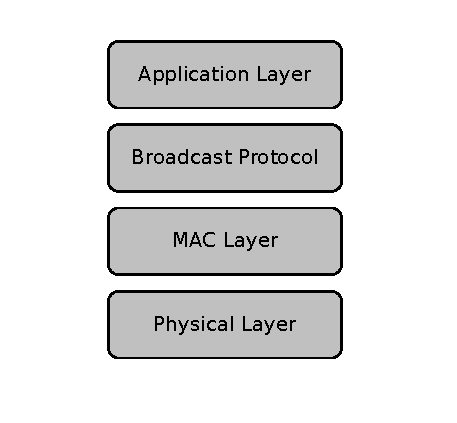
\includegraphics[scale=0.9]{Etat_de_l'art/source/layer.pdf}
\caption{\label{Layer} Les couches dans les WSNs}
\end{figure}

Pour l'étude et la conception d'algorithmes dans les réseaux de capteurs sans fil (WSN), il est indispensable de définir le problème précis, d'établir un cadre rigoureux, formel et sans ambiguïtés. Au vue de la figure \ref{Layer}, notre étude se placera dans la couche 'Broadcast Protocols'. Nous ne développerons pas la couche MAC ni la couche application.\\

La modélisation de base des réseaux de capteurs sans fil \textbf{$M_1$}:
\begin{itemize}
 \item Tout les capteurs sont identiques (batterie, portée, capacité de calcul..).
 \item le réseau est initialement connexe (chaque capteur est lié directement ou indirectement à tout les autres).
 \item Dans un plan euclidien à deux dimensions (distance euclidienne).
 \item Sans mobilité des capteurs : nous supposerons que les capteurs sont immobiles.
 \item Sans ajout de capteurs: le réseau comprend un nombre fixe de capteurs $n$. Aucun ajout de capteurs en cours de fonctionnement n'est possible.
 \item Dans des conditions de transmission de message idéale: aucune interférence entre les messages, pas de perturbations des ondes, système d'identifiants unique.
 \item Fiabilité des capteurs: aucune panne possible, énergie des capteurs infinie .
 \item Chaque site peut a tout moment debuter une procedure de broadcast. Une loi de probabilité modélise ce phénomène.
 \item (Chaque site connait sa position absolue. ) \\
\end{itemize}

  La modélisation \textbf{$M_2$} prendra de plus en compte :
  
\begin{itemize}
 \item Chaque capteur a une énergie initiale $E_i$ donnée. L'envoi de messages consomme une quantité d'énergie en fonction du modèle choisi. Un capteur est éliminé lorsqu'il n'a plus d'énergie ou que son énergie restante ne permet plus aucun envoi de message. Les capteurs ne tombent pas en panne en raison d'autres facteurs.   
 \item L'ajout de capteurs: le réseau comprend un nombre variable de capteurs $n$. Les ajouts de capteurs en cours de fonctionnement sont possibles.\\
 
\end{itemize}

La modélisation \textbf{$M_3$} prendra de plus en compte :

\begin{itemize}
 \item Les capteurs peuvent tomber en panne en raisons de divers facteurs. Une loi de probabilité modélise ce phénomène.   
 \item La mobilité des capteurs.\\
 
\end{itemize}


  Un WSN peut être représenté par un graphe $G= (V,E,\gamma)$ ou $V$ est un ensemble de noeuds (capteurs), $\gamma$ le rayon d'émission maximum et $E \subseteq V \textsuperscript{2}$ l'ensemble des arêtes représentant les communications possibles entre les capteurs: $(u,v)$ appartient à $E$ signifie que $u$ peut envoyer un  message à $v$. On note $ n=|V| $ la taille du WSN. En fait les éléments de E dépendent de la
 position des capteurs ainsi que de leur portée. Nous supposerons que tout les capteurs ont la même portée maximale notée $\gamma$.Nous noterons $ij$ l'arête allant de $i$ à $j$. Nous noterons $d_e(u,v)$ la distance euclidienne dans $\mathbb{R} \textsuperscript{2}$ entre $u$ et $v$.
$$E = \{ (u,v) \in V ^{2} \mid d(u,v) \leq R \}$$

%%%%%%%%%%%%%%%%%%%%%%%%%%%%%%%%%%   Graphe unité
\begin{mydef}
 On appelera $G= (V,E,\gamma)$ le \textit{graphe unité} du WSN et $\gamma$ son rayon de communication.
\end{mydef}

%%%%%%%%%%%%%%%%%%%%%%%%%%%%%%%%%%   Voisinage
\begin{mydef}
On note le 1-voisinage de $u$ : $N_1(u) = \{ v \in V  \mid (u,v) \in E \}$ \\
On note le 2-voisinage de $u$ : $N_2(u) = \{ v \in V \mid  \exists w \in V :\{(u,w);(w,v)\} \in E ^2\}$ \\
On note le $k$-voisinage de $u$, $k \in \mathbb{N} : N_k(u) = \{ v \in V  \mid \exists $ un chemin $c (u,v): |c| \leq k\}$  On parlera de 1- 2- et k-voisins de $i$ pour désigner l'ensemble des noeuds appartenant respectivement à $N_1(i), N_2(i),N_k(i)$. \\
Soit $A \subseteq V$, on note $N(A) = \{ v \in V\textbackslash  A \mid \forall u\in A,(u,v) \in E \}$ \\
\end{mydef}

%%%%%%%%%%%%%%%%%%%%%%%%%%%%%%%%%%   Diametre
\begin{mydef}
 On appelera diamètre de G $diametre_G= \max\limits_{i,j\in \textlbrackdbl 1,n \textrbrackdbl,i<j} (d_G(i,j))$.
\end{mydef}
 

\begin{figure}[H]
\centering
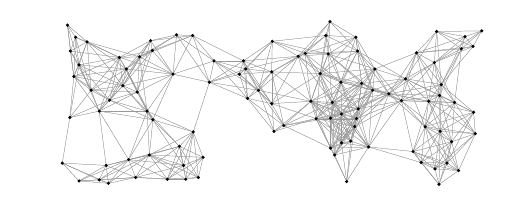
\includegraphics[scale=0.5]{Etat_de_l'art/source/graph1.png}
\caption{Graphe unité}
\end{figure} 

%%%%%%%%%%%%%%%%%%%%%%%%%%%%%%%%%%   Degre
\begin{mydef}
 Le degré de $ u $ est le nombre  $N(u)=|N_1(u)|$.\\
 On note $d(u,v)$ la distance entre $ u $ et $ v $ : $d_G(u,v)= \min\limits_{k \in \mathbb{N}}(k \mid v \in N_k(u))$
\end{mydef}

%%%%%%%%%%%%%%%%%%%%%%%%%%%%%%%%%  Densité, distance moyenne
\begin{mydef}
 La densité de G est la moyenne des degrés:$$N_G=\sum_{i=1}^n{\frac1n N(i)}$$
 La distance de G est la moyenne des distances entre toutes paires de sommets:$$d_G=\sum_{i,j\in \textlbrackdbl 1,n \textrbrackdbl,i<j}{\frac1n d_G(i,j)}$$
 La distance euclidienne de G est la moyenne des distances euclidienne entre toutes paires de sommets:$$d_e(G)=\sum_{i,j\in \textlbrackdbl 1,n \textrbrackdbl,i<j}{\frac1n d_e1(i,j)}$$

\end{mydef}

\subsection{Modèle énergétique}
\subsubsection{Energie d'un capteur}
Tous les capteurs $i$ offrant les mêmes caractéristiques, ils peuvent modifier leur rayon d'émission $r_i$ entre $r_i=0$ et $r_i=\gamma$.
Nous considèrerons que chaque capteur $i$ a une énergie initiale $E_{init}=\beta$.
Nous noterons $E_i$ l'énergie restante de $i$.
L'envoie d'un message de $i$ avec un rayon $r$ coute $$ E(r)= \begin{cases} r^\alpha + c & \text{si }i\neq j \\ 0 & \text{sinon}  \end{cases}$$
L'envoi d'un message de $i$ à $j$ ($d_e(i,j)\leq \gamma$) coûte  $ E_{ij}=E(d_e(i,j))$.
L'énergie consommée lors de la réception de message, du traitement et des calculs propres aux capteurs est négligée.


\subsubsection{Energie globale}
\begin{mydef}
 L'énergie potentielle de G est la somme des énergies des capteurs :$$E_G=\sum_{i=1}^n{E_i}$$
 La consommation de  G est :$$C_G=n\beta - E_G$$
 Le coût moyen de transmition de  G est :$$c_G=E(d_e(G))$$

\end{mydef}

\subsection{Initialisation et mise à jour d'un capteur}
Un capteur 'prend naissance', c'est à dire débute son activité dès qu'il est en place dans le réseaux et ce automatiquement. Deux choix sont possibles: soit le capteur est immédiatement opérationel soit il nécessite une phase 
d'initialisation. Il existe donc deux type d'algorithmes: sans balisage (beaconless) et avec balisage. Les algorithmes 'beaconless' ne nécessitent pas de phase d'initialisation ni de mise à jour. Les nouveaux capteurs sont immédiatement 
opérationels mais n'ont aucune connaissance de leur environnement et notement de leur voisinage dans G. Dans les algorithmes avec balisage, tout capteur, lorsqu'il 'prend naissance' commence par une procédure d'initialisation et stocke en 
mémoire un certain nombre d'informations(voisins,groupe,topologie locale...). Au cour de l'algorithme, chaque noeud met périodiquement à jour ces informations. Pour ce faire chaque site envoie regulierement a ses voisins un message de type
'Hello' contenant par exemple son Id, sa position, sa dominante connexe, son degres, ses voisins, etc.\\
 

Quelle type d'informations est utilisée dans l'algorithme: informations globale du reseau ou informations locales? La distinction entre global est local n'est pas toujours évidente. Des algorithmes centralisés peuvent etre implémentés
 d'une maniere distribuée en décidant par exemple d'un noeud possedant la connaissance globale du réseau.Sinon, au travers d'un échange séquentiel d'informations tres localisées (1 ou 2-voisinage par exemple), chaque noeud peut combiner sa 
connaissance avec celle de ses voisins et ainsi obtenir une vision globale du réseau. Cepandant, une telle phase de propagation coute tres cher en terme de nombre de messages échangés et de temps.
Si le reseau est dynamique (mobilité des capteurs), maintenir une connaissance locale du reseau devient plus complexe tandis que tenir a jour la topologie globale de celui-ci devient impossible par le moyen cité précedement.Ainsi, 
la quantité et la nature des informations nécessaire au déroulement de l'algorithme sont une bonne mesure de la capacité d'adaptation du protocol à un environement dynamique.   

\begin{enumerate}
 \item \textbf{Global}:         protocol de broadcast, centralisé ou distribué nécessitant une connaissance globale du reseau(ex: BIP).
 \item \textbf{Quasi-global}:   protocol distribué de broadcast nécessitant une connaissance quasi-globale du reseau.
 \item \textbf{Quasi-local}:    protocol distribué nécessitant une connaissance du réseau principalement locale et occasionellement globale.
(ex: Cluster networks: tandis que les groupes peuvent etres construits de maniere locale , des reactions en chaines peuvent arrivées).
 \item \textbf{Local}: 		protocol distribué nécessitant une connaissance tres locale du réseau.Tout les algorithmes de 1 ou 2-voisinage appartienent à cette catégorie.
\end{enumerate}


\subsection{Broadcast}

Dans un WSN $G(V,E,\gamma)$, deux capteurs peuvent communiquer directment uniquement si ils sont 1-voisins dans G.
A cause de la perte de propagation des messages, le rayon de transmition est relativement limité, c'est pourquoi les communications doivent se faire par multi-sauts, parfois meme si le destinataire est a distance 1 dans le graphe 
unité(pour des raison énergetiques). Pour établir une connection entre deux noeud non voisins, les messages doivent effectues des sauts via des noeuds intermediaires. Dans un large WSN, il est bien trop difficile pour un capteur voulant
transmettre un message à un autre de trouver une route, à cause de l'absence d'infrastructures. 
La procédure de Broadcast est un mécanisme fondamentale pour la propagation des données ainsi que pour la decouverte de route. C'est pourquoi, concevoir des algorithmes efficaces et economes en énergie est un probleme primordial 
dans les WSN. 





{%
\newcommand{\mc}[3]{\multicolumn{#1}{#2}{#3}}
\begin{center}
\begin{tabular}{|c|l}\cline{1-1}
\mc{2}{c}{\textbf{Notations}}\\\hline
$G(V,E,\gamma)$ & \mc{1}{c|}{Graphe unité}\\\hline
$n$ & \mc{1}{c|}{Nombre de capteur}\\\hline
$\gamma$ & \mc{1}{c|}{Rayon d'émission maximum}\\\hline
$\alpha$ & \mc{1}{c|}{constante de consommation énergetique}\\\hline
$c$ & \mc{1}{c|}{constante de consommation énergetique}\\\hline
$\beta$ & \mc{1}{c|}{Energie initiale des capteur}\\\hline
$E_i$ & \mc{1}{c|}{Energie restante de $i$}\\\hline
$E_{ij}$ & \mc{1}{c|}{Cout d'envoie d'un message de $i$ à $j$}\\\hline
$N(u) $& \mc{1}{c|}{Degre de u}\\\hline
$d_G(i,j)$ & \mc{1}{c|}{distance dans G entre $i$ et $j$}\\\hline
$d_e(i,j)$ & \mc{1}{c|}{distance euclidienne entre $i$ et $j$}\\\hline
$N_k(u)$ & \mc{1}{c|}{nombre de k-voisins de u }\\\hline
$N_G$ & \mc{1}{c|}{densité de G}\\\hline
$d_G$ & \mc{1}{c|}{distance de G}\\\hline
$d_e(G)$ & \mc{1}{c|}{distance euclidienne de G}\\\hline
$diametre_G$ & \mc{1}{c|}{diametre de G}\\\hline
\end{tabular}
\end{center}
}%


\section{Etat de l'Art}\label{class}



\subsection{Algorithmes sans balisage}

\paragraph{Bling Flooding}
Le blind flooding ou broadcast aveugle est un algortihme glouton de broadcast. Lors de la reception d'un message par un noeud, si c'est la premiere fois qu'il le recoit, il le broadcast à ses voivins(avec le rayon maximum), sinon il
 ne fait rien.
\paragraph{Algorithme ABBA}
'Area-based beaconless reliable broadcasting in
sensor networks'\cite{Abba2006}.

L'idée maitresse de ABBA est assez simple. Nous supposons que les noeuds n'ont aucunes connaissance de leur voisinage. Cepandant ceux ci connaissent leurs position géographique (GPS par exemple).
A la premiere réception d'un message, le noeud initialise un timer. Avant expiration du timer, le noeud peut recevoir d'autre copie du meme message. Chaque capteur a un rayon d'emission fixe $R$
et couvre une zone circulaire. Si un noeud $u$ recoit le meme message de differente source et que ces sources couvrent sa zone, alors $u$ ne retransmet pas le message.
Cela signifie que chaqun de ses voisins potentiel a déjà reçu le message. Si un noeud est couvert avant que son timer n'expire, il ne fait rien. Sinon il retransmet.
Comme chaque couverture est un cercle de rayon $R$, le critere de couverture peut etre simplifié: au lieu de s'interesser au disque entier, un noeud verifie uniquement si le perimetre $\pi$ de sa zone est couvert par 
ses voisins lui ayant envoyé le message. 

\begin{algorithm}[h]
\caption{ABBA}
\label{ABBA}
\begin{algorithmic}
\REQUIRE:
Un noeud source $s$, un message $M$
\STATE Reception  par  $u$ du message $M$ venant de $v$
\STATE Calculer la zone $z$ couverte par $v$ lors de la transmittion;
\STATE Déclancher le timer;
\REPEAT
    \STATE Attendre la reception d'un autre copie de $M$ ou que le timer expire;
    \IF {Une copie de $M$ est reçue}
	\STATE Mettre à jour $z$;
	\STATE reinitialiser le timer;
    \ENDIF
\UNTIL{timeout expires;}
\IF {$\pi \nsubseteq z$}
    \STATE Retransmetre;
\ENDIF
     \STATE Ignorer les autres copies de M;

\end{algorithmic}
\end{algorithm}




\subsection{Algorthimes globaux}
\paragraph{Algorithme BIP}
Article \cite{Wieselthier2000}

  Rappelons les desavantages des transmitions longue portée: interférences, cout energetique ( le modele de consommation energetique des noeuds est non linéaire par rapport au rayon à cause de l'attenuation du signal radio).
C'est pourquoi il est necessaire de trouver le bon compromis entre le rayon de transmition et le nombre de messages circulant: un large rayon de transmittion coute cher mais atteind beaucoup de neouds; un court rayon cout tres peu cher mais 
augmente le nombre de messages. 

'Boadcast Incremental Protocol' et glouton et centralisé.Il se base sur l'algorithme de Prim: un algorithme permettant de construire un arbre couvrant minimal d'un graphe. Le principe de l'algorithme de Prim est de construire l'arbre couvrant minimal arête par arête: pour ajouter une 
arête à un arbre partiellement construit, il considère l'ensemble des arêtes dont une extrémité est
connectée à l'arbre déjà construit, et l'autre extrémité ne l'est pas, et
il choisit dans cet ensemble une arête de poids minimal qu'il ajoute à l'arbre. L'algorithme commence avec un arbre couvrant contenant un noeud et zéro arêtes, et ajoute successivement $n-1$ arêtes.

La formation d'un arbre couvrant de poids minimun dans BIP suit le meme principe dans le sens ou les aretes sont une par une ajoutées à l'arbre.
En fait, Bip utilise l'algorithme de Prim avec une difference fondamentale: au lieu d'utiliser des couts fixes $P_{ij}$ sur les aretes (demeurant inchangés au court de la procédure),
Bip actualise dynamiquement ces couts à chaques étapes ($i.e$ à chaque ajout d'une arete), ce qui traduit le fait que le cout d'ajout d'une arete depends des noeuds déja dans l'abre:

$$ \forall i \in BIP, \forall j \notin BIP, P'_{ij}=P_{ij}-P(i)$$
ou $P_{ij}$ est le cout reel de transmition et $P(i)$ le cout de broadcast de $i$ dans l'arbre ( $P(i)=0$ si $i$ est une feuille, $P(i)=\max\limits_{j\in N_1(i)\bigcap BIP}(E_ij)$ sinon ). $P'_{ij}$ represente donc le cout d'ajout de $j$ par un noeud appartenant au sous ensemble des feuilles
directes de $i$(ou $i$ lui meme si c'est une feuille). La paire $\{i,j\}$ minimisant $P'_{ij}$ est selectionnée et $i$ transmet à $j$. Ainsi, une nouveau arete est ajoutée a chaque etape de l'algorithme.\\



\begin{algorithm}[h]
\caption{Procédure de construction du BIP-Tree}
\label{algo_BIP_tree}
\begin{algorithmic}
\STATE ENTREES  $G=(V,E)$ un graphe connexe, $s$ une source
\STATE SORTIE  Arbre BIP de racine s
\STATE B : ENSEMBLE des arêtes de l'arbre
\STATE  $B \leftarrow graphe_{vide}$
\STATE Marquer $s$
\STATE Creer les nouveaux poids: $\forall j \notin BIP, P'_{sj}=P_{sj}-P(s)=P_{sj}$
\WHILE {il existe un sommet non marqué adjacent à un sommet marqué }
   \STATE Mettre à jour les poids:  $ \forall i \in BIP, \forall j \notin BIP, P'_{ij}=P'_{ij}-P(i)$
   \STATE Sélectionner un sommet j non marqué adjacent à un sommet marqué i tel que (i,j) est l'arête sortante de plus faible poids $P'_{ij}$
   \STATE $B := B\bigcup   {(i,j)}$
   \STATE Marquer $j$
\ENDWHILE
\STATE Retourner $B=(V,B)$
\end{algorithmic}
\end{algorithm}

Contairement a Prim qui garantie l'optimalité de l'abre couvrant en termes de cout total,
Bip ne construit pas forcement un arbre de poids minimum. Un fois cet abre construit, le broadcast se fait naturellement via celui-ci.

\begin{algorithm}[h]
\caption{BIP}
\label{algo_BIP}
\begin{algorithmic}
\STATE ENTREES  $G=(V,E)$ un graphe connexe, $s$ une source, un message $M$
\STATE SORTIE  BIP Broadcast
\STATE $s$ envoie $M$ à ses fils dans son Bip-tree
\STATE Lors de reception de $M$ par $i$:
  \IF {$i$ est un noeud} 
    \STATE Retransmettre $M$ à ses fils sinon ne rien faire
\ENDIF
\end{algorithmic}
\end{algorithm}


\subsection{Algorithmes avec balisage}
Comme expliqué en 2.1.3, dans les algorithmes avec balisage, tout capteur, lorsqu'il 'prend naissance' commence par une procédure d'initialisation et stocke en 
mémoire un certain nombre d'informations(voisins,groupe,topologie locale...). Au cour de l'algorithme, chaque noeud met périodiquement à jour ces informations. Pour ce faire chaque site envoie regulierement a ses voisins un message de type
'Hello' contenant par exemple son Id, sa position, sa dominante connexe, son degres, ses voisins, etc.\\
\paragraph{Decouverte 2-voisinnage}

La connaissance du 2-voisinage est un tres bon compromis conservant la localité du protocoles tout en minimisant le nombre de messages.


\begin{algorithm}[h]
\caption{Decouverte k-voisinnage}
\label{algo_k_voisinnage}
\begin{algorithmic}

\FOR{chaque noeud $i$}
	\STATE Broadcaster un message de type <HELLO,$i$> avec un rayon de transmittion $\gamma$
\ENDFOR

\STATE A la réception de <HELLO,$j$> , ajouter $j$ a son 1-voisinage.
\STATE Attendre $\Delta$
\FOR{chaque noeud $i$}
	\STATE Broadcaster <HELLO,$N_1(i)$,$i$>, message contenant $N_1(i)$ le 1-voisinage de $i$
	\STATE A la réception de <HELLO,$N_1(j)$,$j$> , ajouter $N_1(j)$ a son 2-voisinage.
	
\ENDFOR
\end{algorithmic}
\end{algorithm}

Complexité en messages: $O(2n)$.


\paragraph{Algorithme LBIP}  `Localized Broadcast Incremental Power Protocol for Wireless Ad Hoc Networks': article \cite{Ingelrest2004}
LBIP est l'application local de BIP: au lieu de construire l'arbre de diffusion BIP de facon centralisé,il le construit de facon locale.
Chaque site lorsqu'il recoit un message à retransmettre calcul son BIP-tree sur son 2-voisinage et diffuse le message par l'intermediaire de celui ci.

\begin{algorithm}[h]
\caption{LBIP}
\label{algo_LBIP}
\begin{algorithmic}
\STATE ENTREES  $G=(V,E)$ un graphe connexe, $s$ une source, un message $M$
\STATE SORTIE  LBIP Broadcast
\STATE REQUIE  Connaissance du 2-voisinage
\STATE $s$ calcul son arbre et diffuse <MSG,$s$> à ses fils
\IF{ $u$ recoit <MSG,$v$> :}
	\IF{Le paquet contient des instruction pour $u$}
		\STATE $u$ construit son 2-BIP-tree est retransmet le message à ses fils
	\ENDIF
\ENDIF
\end{algorithmic}
\end{algorithm}


\paragraph{Algorithme DLBIP}
`Dynamic Localized Broadcast Incremental Power Protocol for Wireless Ad Hoc Networks': article\cite{Champ2009DLBIP}.
DLBIP est une amélioration de LBIP. Le principe est de repartir l'energie consommée lors d'un broadcast en empreintant des chemins (arbre couvrants) différents en fonction de l'energie restantes des noeuds qui vont servir de relais.
A chaque broadcast, l'abre de diffusion est recalculé sur le meme graphe mais avec de nouveaux poids dépendants de l'energie de communication entre les noeuds ainsi que de l'energie propre à chaque noeud. Ce protocols permet que
le niveau d'energie propre à chaque noeud baisse globalement de façon identique et ainsi retarder un maximum la panne d'un capteur par manque d'energie.


.............................Algo a faire
\begin{algorithm}[h]
\caption{DLBIP}
\label{algo_DLBIP}
\begin{algorithmic}
\STATE ENTREES  $G=(V,E)$ un graphe connexe, $s$ une source, un message $M$
\STATE SORTIE  DLBIP Broadcast
\STATE REQUIE  Connaissance du 2-voisinage
\STATE $s$ calcul son arbre et diffuse <MSG,$s$> à ses fils
\IF{ $u$ recoit <MSG,$v$> :}
	\IF{Le paquet contient des instruction pour $u$}
		\STATE $u$ construit son 2-BIP-tree est retransmet le message à ses fils
	\ENDIF
\ENDIF
\end{algorithmic}
\end{algorithm}



\paragraph{Algorithme RRS}
\cite{Cartigny2003RNG}
\subsubsection{Algorithme RBOP}
\cite{Cartigny2005}
\begin{figure}[H]

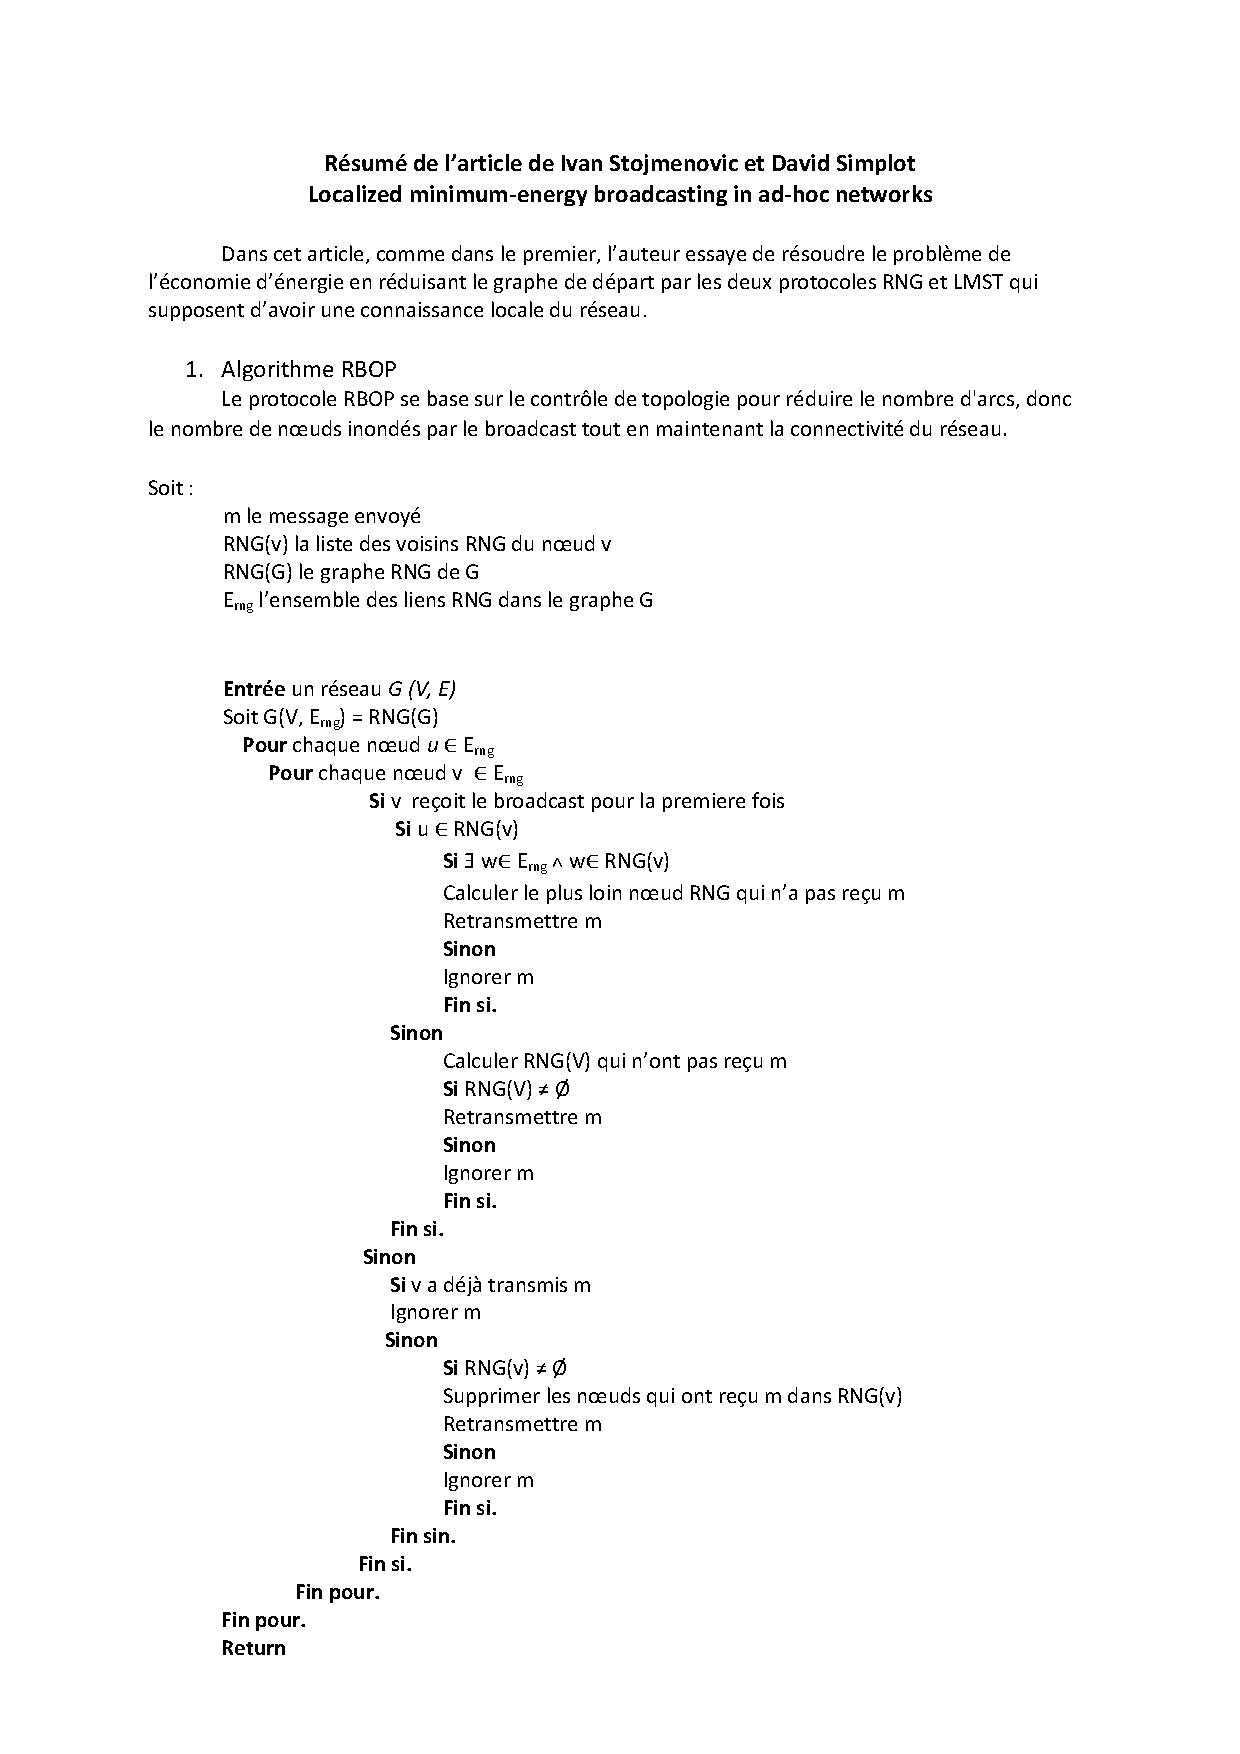
\includegraphics[scale=1]{Etat_de_l'art/source/RBOP}

\end{figure} 


\subsubsection{Algorithme LBOP}
\cite{Cartigny2005}
\subsubsection{Algorithme DLBOP}
\cite{Cartigny2004}
\subsubsection{Algorithme TR-LBOP}
\cite{Ingelrest2004}
\subsubsection{Algorithme FONIA}

\subsubsection{Algorithme Dominating set}
In a {\it reliable} protocol, every node in the network is reached. The set of nodes that rebroadcast message in a reliable broadcasting scheme 
define a connected dominating set. A dominating set $D(S)$ of a set $S$ is a set of nodes such that each node fiom $S$ either belongs to $D(S)$ or has a neighboring node that belongs to $D(S)$. It is easy to observe that all
 nodes will receive the message if it is retransmitted only by nodes that belong to a connected dominating set. Connectivity provides propagation through the whole network, while domination assures reachability by all nodes.
 Broadcasting task can therefore be solved optimally by finding a connected dominating set of minimal size. Optimality here is measured by percentage of saved retransmissions in a reliable broadcasting scheme. Unfortunately,
 the problem of finding connected dominating set of minimal size is NP-complete, even if a node has global knowledge about the network [HH, LK, QVL]. Therefore one needs to apply heuristics to flood intelligently. Note also
 that a protocol that is reliable on the network layer may be very unreliable at the MAC layer, such as blind flooding. Excess messages in any protocol affect node's power and bandwidth available, thus the main goal is to
 describe a reliable broadcast protocol with minimal number of retransmissions, that is, to construct connected dominating set of minimal size. Note also that MAC layer cannot guarantee 100\% reliability, due to the hidden
 terminal problem (a node simultaneously receiving messages fiom two other nodes that are not aware of each other transmission) and the probabilistic nature of protocols used.

\subsection{Probalistics}


\subsubsection{Algorithme BWGOSSIP}
\cite{lutzeler2011}
\subsubsection{Algorithme Duty-Cycle-Aware Broadcast in WSN }
\cite{Wang2009},\cite{Wang2010}
\subsubsection{Algorithme HEED}
\cite{Younis2004}
\subsubsection{Algorithme WMH}
\cite{Agarwal2005}
\subsubsection{Algorithme IRRIGATOR  Firework}
\cite{orecchia2004}
\subsubsection{Algorithme ML2B}
\cite{zhaobroadcast}
\subsubsection{Algorithme MLE}
\cite{Cheng2006}
\subsubsection{Algorithme MPR}

\subsubsection{Algorithme Power Adaptive Broadcasting with Local Information}
\cite{Chen2003}



\subsection{Protocoles}
\subsubsection{NES}


\subsection{Elements de classification}
Les éléments de classification cités ci dessous sont inspirés des articles \cite{stojmenovic2004},\cite{ingelrest2005},\cite{wu2003}
\begin{enumerate}
 \item  \textbf{Extensibilité}: Pour qu'un protocol soit extensible, il doit etre avant tout distribué et local: le comportement de chaque noeud bien qu'il
nécessite qu'une connaissance locale du reseau, permet d'atteindre l'objectif global. Il est facile d'admettre que l'extensibilité d'un WSN est inversement proportionelle à la localité du protocol. 
 \item  \textbf{Connectivité}: La connectivité d'un algorithme mesure se capacité à atteindre tout les sites.
 \item  \textbf{Deterministe vs probabiliste}: Un protocol de broadcast peut utiliser des fonctions probabilistes pour prendre certaines descisions de maniere aléatoire.
 \item  \textbf{Rayon d'émission}:  rayon fixe ou variable
 \item  \textbf{Avec ou sans balisage}:  
 \item  \textbf{}:  
 \item  basé sur les clusters
 \item  Grid Partitioning-Based Backbone
 \item  Connected Dominating Set (CDS)-Based Backbone
 \item  Activity scheduling and power-aware broadcasting
 \item  Broadcasting with directional antennas
 \item  Flooding scheme 
 \item  Probabilistic flooding
 \item  1-Hop Neighbor Knowledge Methods
 \item  Flooding with Self Pruning (FSP)
 \item  2-Hop or More Neighbor Knowledge Methods
 \item  Multipoint Relaying (MPRs)
 \item  Using Connected Dominating Set (CDS)
 \item  Area Based Methods.....................
 
\end{enumerate}


\newpage
\subsection{Synthèse}



\newpage

\begin{figure}[H]
\centering
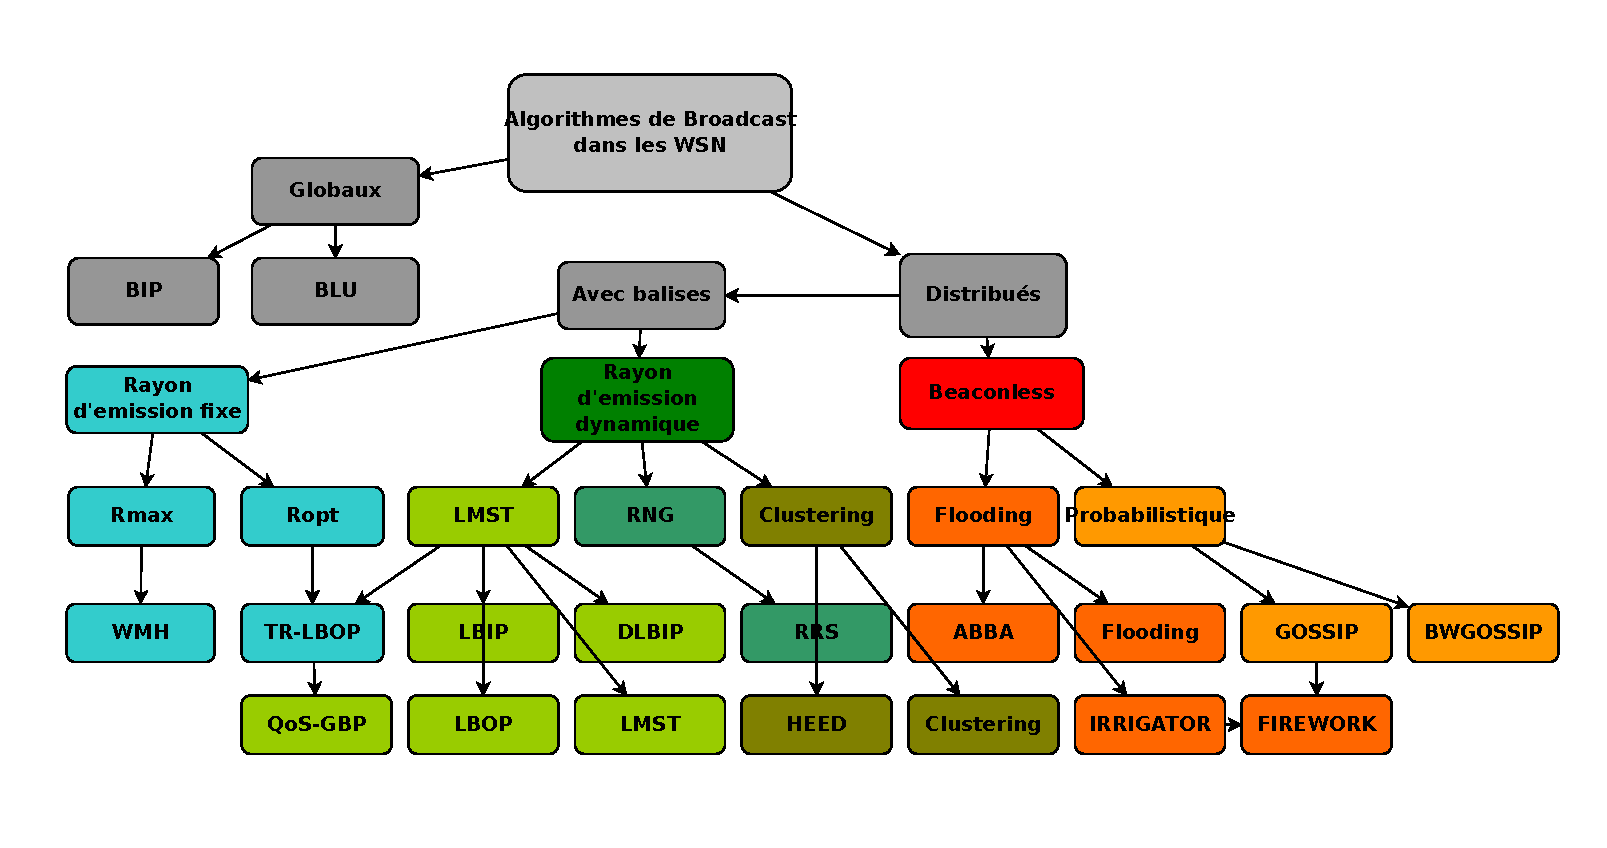
\includegraphics[scale=1,angle=90]{Etat_de_l'art/source/classification}
\caption{Description, Figure 1 : Graphe de synthèse}
\end{figure} 


